% HAND-AUTHORED grouped bar plot of the data in figures/scaling-table.tex
% (auto-generated from extra/artifacts/rv2026-eval/e4/scaling_merged.json
% by e4_merge_scaling.py, tidystl repo). Update both together; the emitter
% does not yet produce this plot. Times in ms; RTAMT batched values are
% N x per-trace (dagger); STLCG++ OOMs at T=5001 (missing bars).
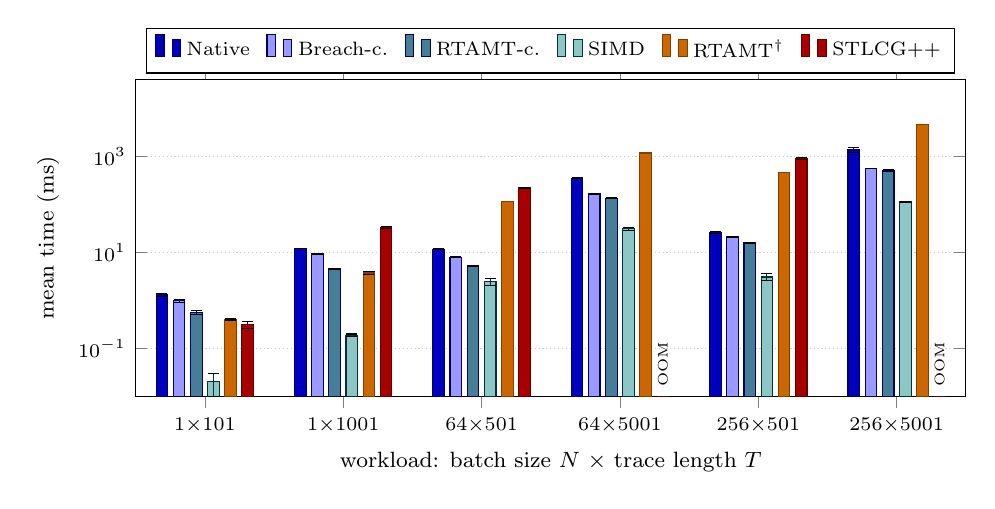
\begin{tikzpicture}
\begin{axis}[
  ybar,
  ymode=log,
  log origin=infty,
  width=\textwidth,
  height=5.6cm,
  bar width=4.2pt,
  ymin=0.01, ymax=40000,
  enlarge x limits=0.10,
  symbolic x coords={1x101,1x1001,64x501,64x5001,256x501,256x5001},
  xtick=data,
  xticklabels={
    {$1{\times}101$},{$1{\times}1001$},{$64{\times}501$},
    {$64{\times}5001$},{$256{\times}501$},{$256{\times}5001$}},
  xlabel={workload: batch size $N$ $\times$ trace length $T$},
  ylabel={mean time (ms)},
  legend columns=6,
  legend style={at={(0.5,1.02)}, anchor=south, font=\scriptsize,
    /tikz/every even column/.append style={column sep=4pt}},
  tick label style={font=\scriptsize},
  label style={font=\footnotesize},
  ymajorgrids,
  grid style={densely dotted, gray!40},
  error bars/y dir=both,
  error bars/y explicit,
]
% tidySTL backends (cool colors)
\addplot[fill=blue!75!black, draw=blue!40!black] coordinates {
  (1x101,1.30) +- (0,0.08) (1x1001,12.15) +- (0,0.19)
  (64x501,11.75) +- (0,0.25) (64x5001,358) +- (0,11)
  (256x501,26.19) +- (0,1.54) (256x5001,1377) +- (0,155) };
\addplot[fill=blue!40, draw=blue!40!black] coordinates {
  (1x101,0.98) +- (0,0.06) (1x1001,9.34) +- (0,0.28)
  (64x501,7.94) +- (0,0.15) (64x5001,167) +- (0,6)
  (256x501,21.42) +- (0,0.65) (256x5001,569) +- (0,9) };
\addplot[fill=cyan!55!black, draw=blue!40!black] coordinates {
  (1x101,0.57) +- (0,0.06) (1x1001,4.58) +- (0,0.08)
  (64x501,5.24) +- (0,0.20) (64x5001,136) +- (0,2)
  (256x501,15.97) +- (0,0.37) (256x5001,515) +- (0,23) };
\addplot[fill=teal!45, draw=teal!40!black] coordinates {
  (1x101,0.02) +- (0,0.01) (1x1001,0.19) +- (0,0.01)
  (64x501,2.44) +- (0,0.41) (64x5001,31.20) +- (0,1.89)
  (256x501,3.09) +- (0,0.50) (256x5001,115) +- (0,2) };
% real tools (warm colors)
\addplot[fill=orange!80!black, draw=orange!50!black] coordinates {
  (1x101,0.40) +- (0,0.01) (1x1001,3.74) +- (0,0.28)
  (64x501,118) (64x5001,1195) (256x501,471) (256x5001,4781) };
% OOM rows carry a zero-height phantom bar (y = ymin) whose node-near-coord
% prints the label exactly in the STLCG++ bar slot.
\addplot[fill=red!65!black, draw=red!40!black,
  point meta=explicit symbolic,
  nodes near coords,
  every node near coord/.append style={
    rotate=90, anchor=west, font=\tiny, text=black},
] coordinates {
  (1x101,0.31) +- (0,0.05) []
  (1x1001,33.71) +- (0,1.31) []
  (64x501,224) +- (0,3) []
  (64x5001,0.01) [OOM]
  (256x501,934) +- (0,44) []
  (256x5001,0.01) [OOM] };
\legend{Native, Breach-c., RTAMT-c., SIMD, RTAMT$^\dagger$, STLCG++}
\end{axis}
\end{tikzpicture}%
